\section{Ejercicio 1: Consultando Datos} 


\textbf{}\\
\textbf{}\\
Paso 1.Ingresar a Visual Studio y abrir o generar el proyecto que genera el contexto EF6-Code-First-Demo.

Paso 2. Agregar a la solución un Proyecto de pruebas unitarias .Net Framework.

\begin{center}
	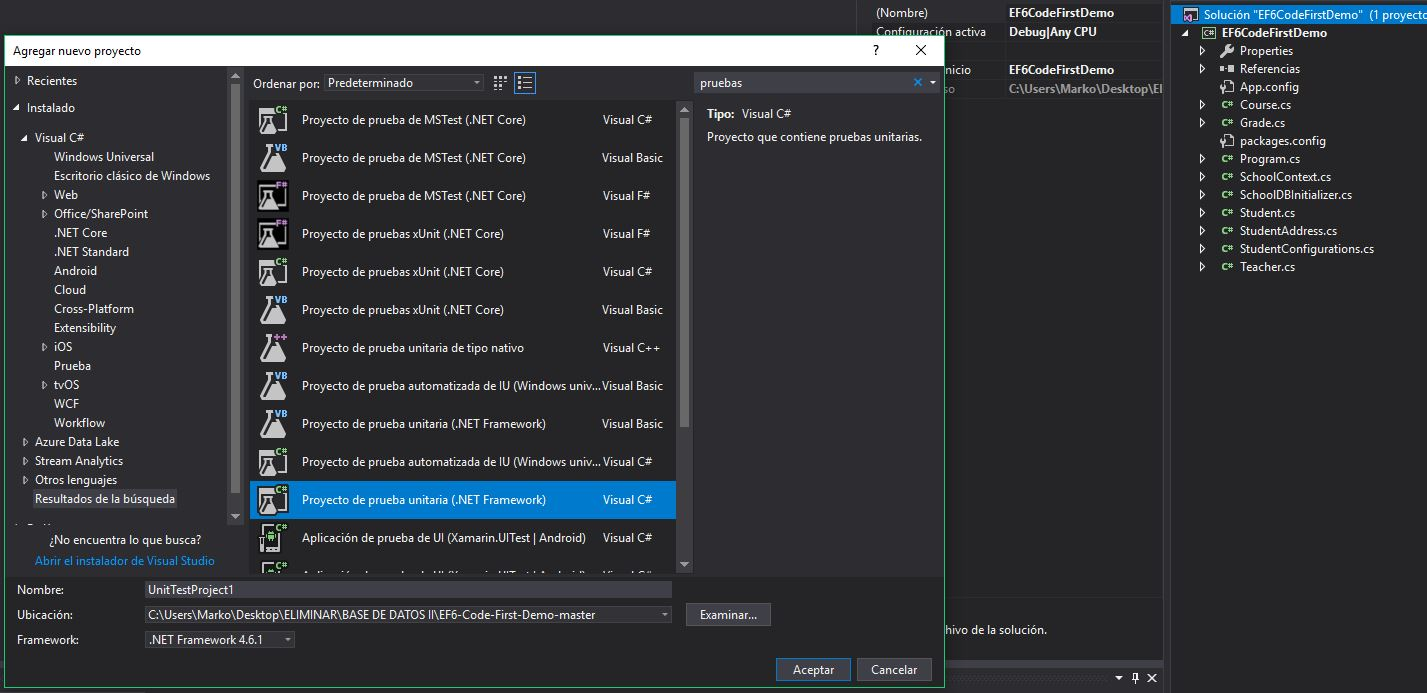
\includegraphics[width=10cm]{./Imagenes/Captura1} 
	\end{center}

Paso 3. En el proyecto de pruebas referenciar al proyecto principal al proyecto de pruebas

\begin{center}
	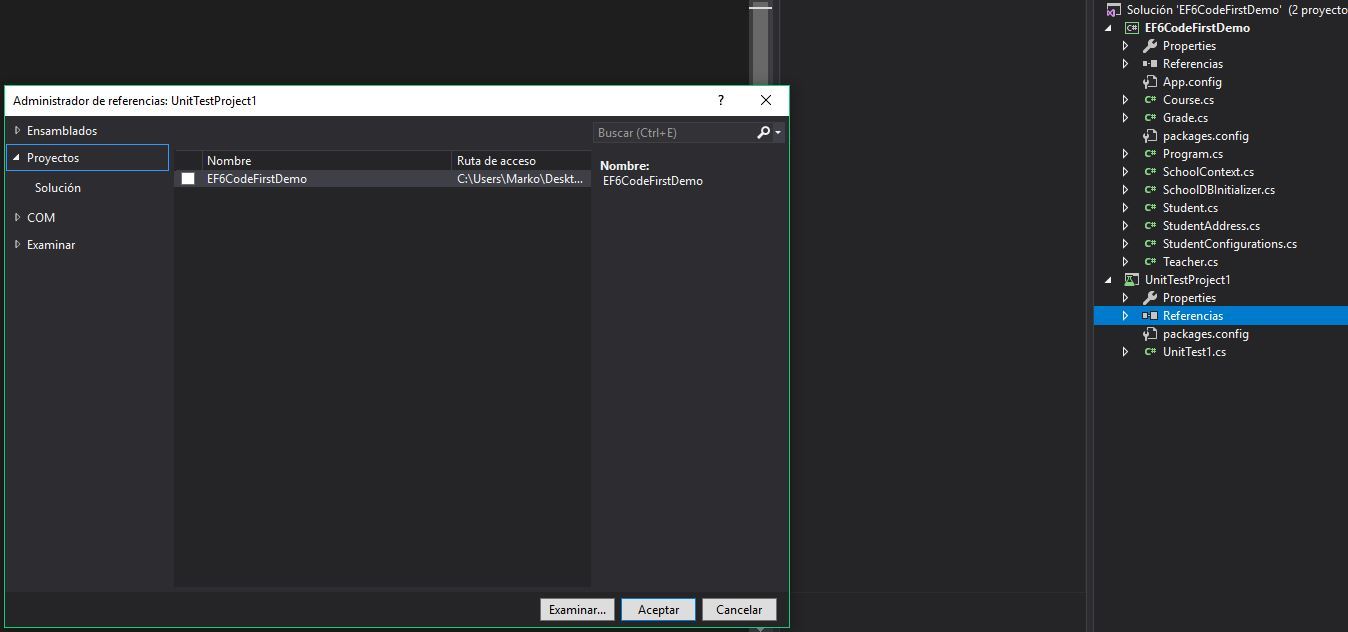
\includegraphics[width=10cm]{./Imagenes/Captura2} 
	\end{center}
Paso 4. En la clase Unitest generada crear el método: ObtenerAlEstudianteConIDUno, puede tomar como
referencia el siguiente código

\begin{center}
	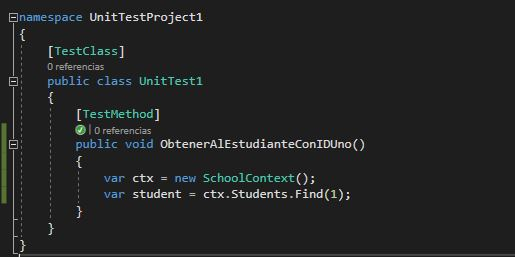
\includegraphics[width=10cm]{./Imagenes/Captura3} 
	\end{center}

\textbf{}\\
La sentencia SQL generada del lado del gestor de base de datos es: 

\begin{center}
	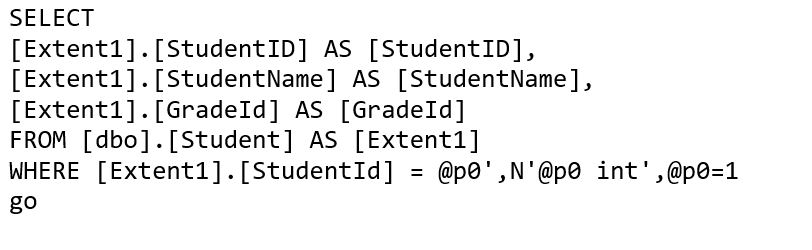
\includegraphics[width=10cm]{./Imagenes/U1-1} 
	\end{center}
\textbf{}\\

Paso 5. Adicionar otro método: BuscarAlPrimerEstudianteConElNombreBill, puede tomar como referencia el
siguiente código.

\begin{center}
	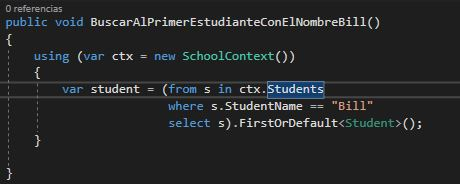
\includegraphics[width=10cm]{./Imagenes/Captura4} 
	\end{center}
\textbf{}\\

La sentencia SQL generada del lado del gestor de base de datos es: 

\begin{center}
	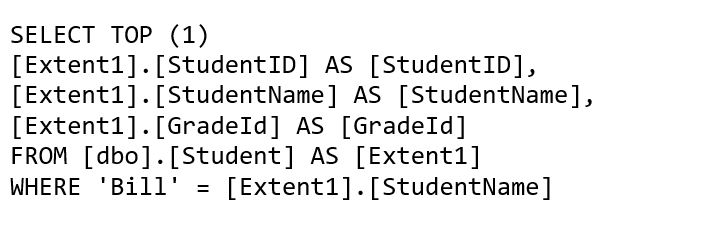
\includegraphics[width=10cm]{./Imagenes/U1-2} 
	\end{center}
\textbf{}\\
Paso 6. Agregar otro método de prueba denominado: BuscarEstudiantesAgrupadosPorGrado, tomar como
referencia el siguiente código.

\begin{center}
	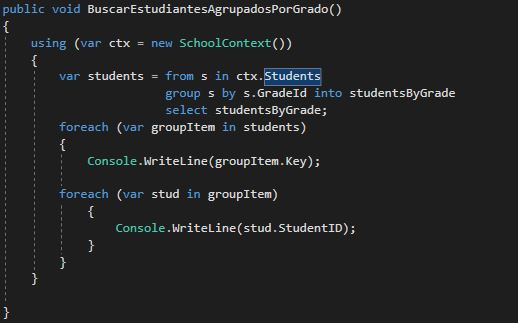
\includegraphics[width=10cm]{./Imagenes/Captura5} 
	\end{center}
\textbf{}\\

La sentencia SQL generada del lado del gestor de base de datos es: 


\textbf{}\\

Paso 7. Agregar otro método de prueba denominado: ObetenerListadoDeEstudiantesOrdenadosPorNombre, tomar
como referencia el siguiente código.

\begin{center}
	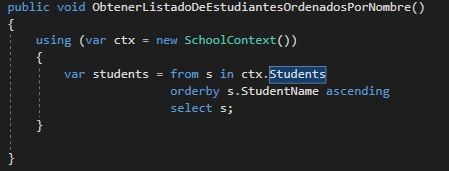
\includegraphics[width=10cm]{./Imagenes/Captura6} 
	\end{center}
\textbf{}\\

La sentencia SQL generada del lado del gestor de base de datos es: 

\begin{center}
	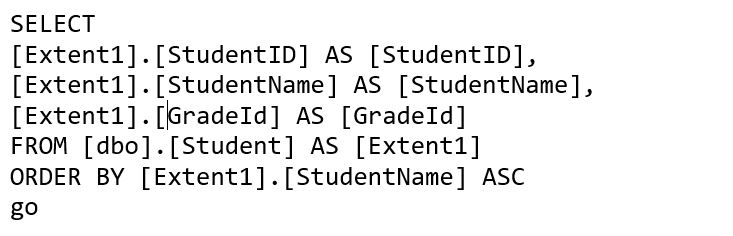
\includegraphics[width=10cm]{./Imagenes/U1-4} 
	\end{center}
\textbf{}\\

Paso 8. Finalmente crear el método de prueba: BuscarTodosLostudiantesConElEstandarUno, tomar como
referencia el siguiente código.

\begin{center}
	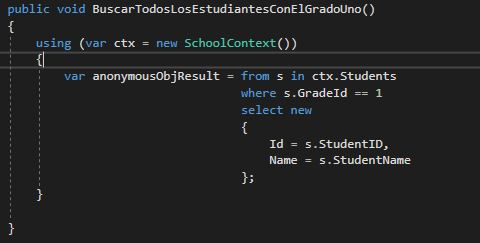
\includegraphics[width=10cm]{./Imagenes/Captura7} 
	\end{center}
\textbf{}\\

La sentencia SQL generada del lado del gestor de base de datos es: 

\begin{center}
	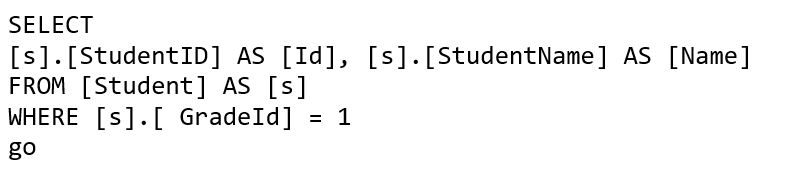
\includegraphics[width=10cm]{./Imagenes/U1-5} 
	\end{center}
\textbf{}\\

\textbf{}\\
